%!TEX root = Abschluss-ML-Prak-2015.tex
\section{Sliding Window}

\subsection{Sliding Window}

\begin{frame}{Sliding Window}
  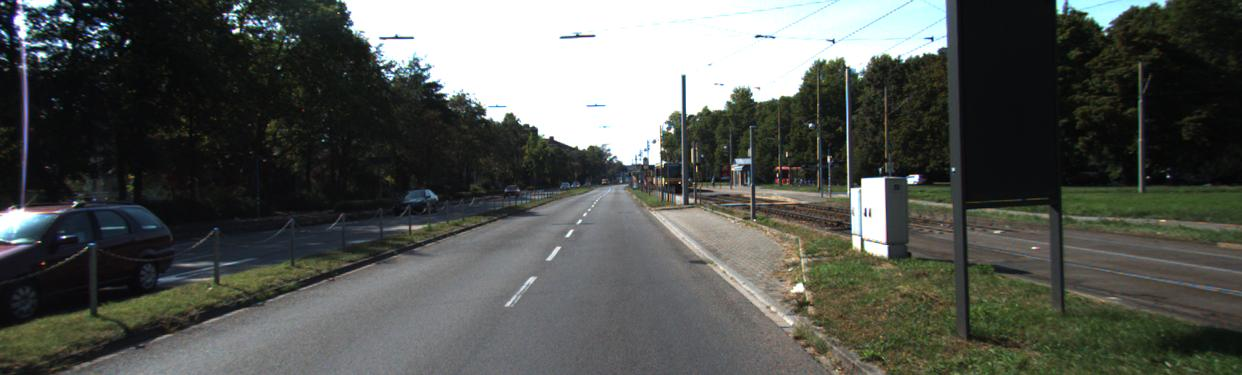
\includegraphics[scale=0.11]{../images/Lasagne/padded.jpg}
  \hspace{0.1cm}
      
\includegraphics[scale=0.12]{../images/Lasagne/29x29-color-coordinates.jpg}
         \vspace{0.1cm}
    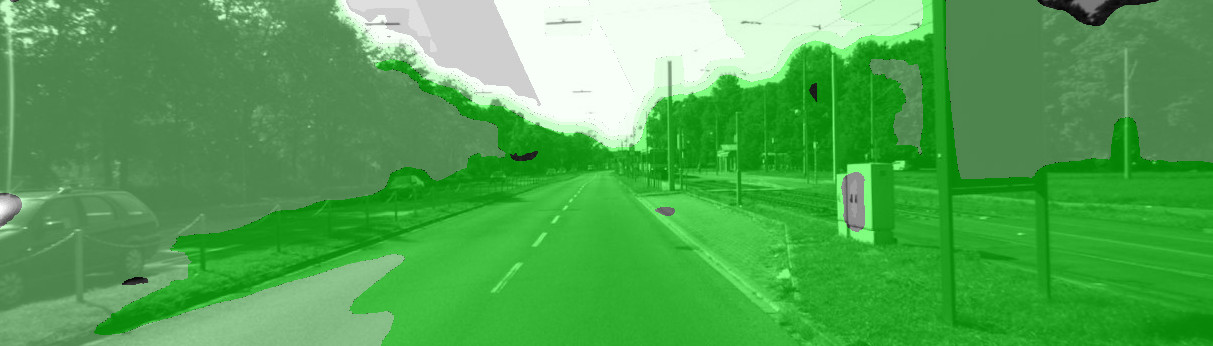
\includegraphics[scale=0.2]{../images/Lasagne/29x29-color-coordinates-overlay.jpg}
         \begin{itemize}
       \item Implementierung mit Lasagne, Windowsize 29~Pixel
        \item Pixelkoordinate als zusätzliches Feature
    \end{itemize}
  $\rightarrow$ \emph{schlechte Ergebnisse}, \emph{lange Laufzeit}

\end{frame}

\section{Ausblick}
\subsection{Ausblick}
\begin{frame}{Ausblick}
    \begin{itemize}
        \item Siliding Window Ansatz nicht weiterverfolgen
        \item in Kontakt mit Jonathan Long, bzgl. Caffe Implementierung
        \item Fully Concolutional Networks mit Lasagne implementieren
    \end{itemize}
    Davon erhoffen wir uns:
    \newline
    $\rightarrow$ \emph{flexible Anpassung},  \emph{schnellere Laufzeit} und  \emph{gute Resultate}
\end{frame}